%!TEX root = ../dokumentation.tex

\chapter{Theoretische Grundlagen}\label{cha:Grundlagen}
Für die Erstellung der App, sowie für die Auswahl der Sensoren und Erstellung des Messaufbaus ist verschiedenes Wissen notwendig. Diese theoretischen Grundlagen werden im folgenden erläutert. 

\section{Luftqualität}\label{sec:Luftqualität}
Die Luftqualität gibt den Gütegrad der Luft an.  Dabei handelt es sich um die Bewertung und den Einfluss von Verunreinigung durch Fahrzeugabgase oder Kraftwerke. Bestandteile der ausgestoßenen Luft, wie beispielsweise \acf{NOx} oder Feinstaub, sind für die Luftverschmutzung verantwortlich und werden in Kapitel? näher erläutert.
Um die Luftqualität möglichst hoch zu halten und den Menschen wenig zu schaden werden Richtlinien mit Grenzwerten eingeführt sowie fortlaufend verfeinert. Diese Richtlinien geben die Höhe sowie deren Eintrittshäufigkeit pro Zeiteinheit an. Das überschreiten der Grenzwerte hat Sanktionen zur Folge. 
\subsection{Indices}
Zur allgemeingültigen Bewertung der Luft gibt es diverse Luftqualitätsinidices, die basierend auf den gemessenen Werten von Feinstaub (PM2,5 und PM10), bodennahem \acf{O3}, \ac{NO2} und \acf{SO2}, den Gütegrad der lokalen Luft bestimmen. Zur Messung dieser Werte werden derzeit meist stationäre Sensoren, oftmals an viel befahrenen Straßen, eingesetzt. 
\newline
Es gibt Länder- und Regionenspezifische Indices. Im folgenden werden die Indices für Europa und für die Vereinigten Staaten erläutert.

\subsubsection{\acf{AQI}}
Der sogenannte \acf{AQI} bildet für die Vereinigten Staaten eine Skala von 0 bis 500 ab. Mit steigendem Wert wird die Luftqualität, bezogen auf den Tag, schlechter und die Risiken für den Menschen schwerwiegender. Die folgende Tabelle stellt die Zusammenhänge von \acs{AQI}-Wert und den Folgen sowie deren Bedeutung dar. Laut \acf{EPA} ist ein Wert von maximal 100 als gesundheitlicher Standard angesetzt.
\newline
\begin{table}[H]
	\begin{center}
		\resizebox{\columnwidth}{!}{%
		\begin{tabular}{|c|c|c|}
			\hline
			Air Quality Index Levels of Health Concern & Numerical Value & Meaning\\ \hline \hline
			Good & 0 to 50 & Air quality is considered satisfactory, and air pollution poses little or no risk. \\ \hline 
			Moderate & 51 to 100 &  	Air quality is acceptable; however, for some pollutants there may be a moderate health concern for a very small number of people who are unusually sensitive to air pollution.\\ \hline
			Unhealthy for Sensitive Groups & 101 to 150 & Members of sensitive groups may experience health effects. The general public is not likely to be affected. \\ \hline
			Unhealthy &  151 to 200 & Everyone may begin to experience health effects; members of sensitive groups may experience more serious health effects.\\ \hline
			Very Unhealthy & 201 to 300 & Health alert: everyone may experience more serious health effects. \\ \hline
			Hazardous & 301 to 500 & Health warnings of emergency conditions. The entire population is more likely to be affected. \\ \hline	
		\end{tabular}
	}
	\end{center}
	\caption{\acs{AQI} Übersicht}
\end{table}

\subsubsection{\acf{CAQI}}
Europäische Länder haben eine eigene, angepasste Skala zur Bewertung der Luftqualität: den \acf{CAQI}. Man unterscheidet hierbei kurzfristige (stündlich oder täglich) von langfristigen (jährlich) Luftqualitätsindices. 
Die stündlich und täglich aktualisierte Luftverschmutzung wird als relatives Maß aus den für Europa bedeutendsten Schadstoffen. Dazu gehören der Feinstaub (PM2,5 und PM10), \acs{NO2} und \acs{O3}. Bei entsprechend verfügbaren Daten können ebenfalls \acf{CO} sowie \acs{SO2} einbezogen werden. Zur Berechnung der Index-Klasse unterscheidet man zwischen dem Verkehrs- sowie dem Hintergrundindex. Ersteres soll die Verkehrsbelastung anhand Messsensoren in direkter Nähe von vielbefahrenen Straßen und letzteres die allgemeine Belastung einer Stadt darstellen. 
\newline
Über den für ein ganzes Jahr hinweg berechneten Index lässt sich der Abstand zu den EU-Grenzwerten darstellen. Der Schwellwert ist dabei 1. Ein höherer Wert des Luftqualitätsindex zeugt von einer Überschreitung eines oder mehrerer Schadstoffwerte. Die Vergleichswerte entsprechen einer Empfehlung durch die Welt Gesundheitsorganisation und dienen dem Schutz der Gesundheit. 
\newline
Die aktuellen Luftqualitätswerte der Messstationen Europas werden von der EUA und der Europäischen Kommission online unter 
\subsection{Schadstoffe}
Im Folgenden soll auf messbare und für die Luftqualität bzw. die menschliche Gesundheit entscheidende Schadstoffe eingegangen werden. Neben der Erläuterung der luftverunreinigenden Teilchen wird auch auf deren Konsequenzen für den Menschen eingegangen. 
\subsubsection{Feinstaub}
Ein für die Gesundheit des Menschen entscheidender Schadstoff ist der Feinstaub oder auch Schwebstaub genannt. Diese kleinen, für das menschliche Auge nicht sichtbaren Teilchen, die nur langsam zu Boden sinken, sind zum größten Teil menschlicher Herkunft. Dazu gehören die Emissionen, die durch Kraftfahrzeuge, Öfen und Heizungen in Innenräumen sowie durch die Metallerzeugung, auftreten. Dabei wird der durch Kraftfahrzeuge entstehende Feinstaub nicht nur aus dem Motor emittiert, sondern auch Bremsen- und Reifenabrieb sowie die Aufwirbeln des Straßenstaubes verunreinigen die Luft. Die eben genannten Faktoren tragen zum primären Feinstaub bei. Der sekundäre Feinstaub hat seine Herkunft in der Landwirtschaft. Hierbei entstehen in der Tierhaltung gasförmige Schadstoffe durch die Ammoniakemissionen. 
\newline
Dabei unterteilt man die Partikel nach ihrer Größe. Alle Teilchen mit einem aerodynamischen Durchmesser kleiner 10 Mikrometer werden als PM10, wobei man diejenigen mit einem Durchmesser von kleiner 2,5 Mikrometer als PM2,5 bezeichnet. Eine weitere Aufschlüsselung innerhalb der eben genannten Grenzen ergibt die Begrifflichkeiten Grobfraktion, für alle Partikel zwischen 2,5 und 10 Mikrometer, sowie die Feinfraktion, für Partikel mit einem Durchmesser kleiner 2,5 Mikrometer. Die allerkleinsten Partikel, aerodynamischer Durchmesser kleiner als 0,1 Mikrometer nennt man ultrafeine Partikel. PM10 wandern in die Nasenhöhlen, PM2,5 gelangen über die Atemwege in die Bronchien sowie Lungenbläschen und setzen sich dort ab. Die ultrafeinen Partikel können bis in die Blutgefäße eindringen können. Als Folgen können abhängig von der Partikelgröße Atembeschwerden entstehen sowie die Gefahr eines Herzinfarkts oder einer Lungenerkrankung steigen. 

\subsubsection{\acs{NOx}}
Stickstoffoxide sind die Verbindung aus unterschiedlich vielen Stickstoff- und Sauerstoffatomen. Die wichtigsten Vertreter dieser Gruppe sind das Stickstoffmonoxid und das Stickstoffdioxid. Diese Oxide entstehen bei unerwünschten Nebenreaktionen während der Verbrennung von Benzin, Öl, Gas oder Kohle. Sie stellt einen sehr reaktionsfreudigen Stoff dar, wodurch es nicht nur zur Ozonbildung, sondern auch zur Feinstaubbelastung beiträgt. 
\newline
Stickstoffdioxide können vor allem bei Asthmatikern zur Bronchienverengung führen. 

\subsubsection{\acs{SO2}}
Das farblose aber stark riechende Schwefeldioxid wird vor allem bei der Verbrennung von Kohle oder Öl erzeugt und liegt im Normalfall als Gas vor. 
\newline
Für den Menschen hat dieser Schadstoff Schleimhaut- und Augenreizungen sowie Atemwegsprobleme zur Folge. 
\newline
Heutzutage ist die Belastung durch SO2 jedoch nicht mehr kritisch und die Gesundheitsrisiken akut nicht vorhanden.
\newline
Zudem entstehen aus Schwefeldioxid Sulfatpartikel in der Atmosphäre, die die PM10 Belastung verstärken. 

\subsubsection{\acs{O3}}
Bodennahes \acs{O3} gilt als sekundärer Schadstoff, da es erst durch photochemische Prozesse entsteht und nicht direkt emittiert wird. Es ergibt sich vor allem aus \acs{NOx} sowie flüchtigen organischen Verbindungen. Diese beiden sogenannten Vorläuferstoffe werden überwiegend vom Menschen erzeugt. Während \acs{NOx} von Kraftfahrzeugen emittiert werden, entstehen flüchtige organische Stoffe bei der Verwendung von Lösemitteln, wie zum Beispiel in Farben, Klebstoffen, Reinigungsmitteln oder durch die Verbrennung von Kraftstoff. 
\newline
Zu den gesundheitlichen Folgen gehören eine geringere Lungenfunktion sowie Atemwegsbeschwerden. Diese Wirkungen treten vor allem bei körperlicher Belastung sowie bei besonderes anfälligen oder vorgeschädigten Personen auf. 

\subsubsection{\acs{CO}}
Das gasförmige, farb- und geruchslose \acs{CO} wird bei der unvollständigen Verbrennung von Kraftstoffen freigesetzt. Der Grund hierfür ist Sauerstoffmangel, der bei extrem niedriger Dosierung zu einer \acs{CO} Konzentration fährt und in einem solchen Fall als Atemgift wirkt. Das liegt an der Beeinträchtigung der Sauerstoffaufnahme und zieht negative Konsequenzen für das zentrale Nervensystem mit sich. 
\newline
Des Weiteren ist \acs{CO} ein Bestandteil bei der Bildung von bodennahem \acs{O3}. 

\subsubsection{\acl{CO2}}
\acs{CO2} ist ein farb- und geruchsloses Gas. Es ist als Treibhausgas für das auf der Erde entstehende Klima verantwortlich, indem es einen Teil der Wärme, die ins Weltall ausgestrahlt wird zurück auf die Erde emittiert. Neben den großen Vorkommnissen im Weltall wird es ebenfalls bei der Zellatmung von Menschen und vielen Tieren ausgeschieden. Ein weiterer Entstehungsort ist der Verbrennungsvorgang von Öl, Holz oder Kohle. Ein Problem von \acs{CO2}, ist dass sich dieser Schadstoff nicht selbstständig wieder abbauen kann. Die einzige Möglichkeit zur Reduzierung des \acs{CO2}-Gehaltes ist die Photosynthese oder die physikalische Speicherung in Gewässern. Dabei entsteht Glucose und Sauerstoff. 
\newline
Die folgende Tabelle zeigt die Auswirkungen von diversen \acs{CO2}-Konzentration auf den Menschen.


\section{Hardware}\label{sec:Hardware}
Um die Luftqualität in verschiedenen Luftschichten messen zu können ist diverse Hardware notwendig. 
\newline
Für die Messung werden unterschiedliche Sensoren benötigt, die die wichtigsten Aspekte der Luftqualität, wie zum Beispiel den Feinstaub, messen. 
\newline
Um die Daten zu verarbeiten und auszulesen ist ein µ-Controller notwendig. In dieser Arbeit wurde ein XDK der Firma Bosch verwendet. 
\newline
Um agil messen zu können wird eine Drone der Marke DJI eingesetzt. Die Modellbezeichnung lautet Phantom 3 Standard.

\subsection{DJI Phantom 3 Standard}\label{subsec: Phantom 3}
Der Aufbau der Drone ist in folgender Abbildung zu sehen. Die Drone hat vier Propeller, welche die Antriebskraft leisten. Um Bilder und Videos aufzunehmen ist auf der Unterseite der Drone ein Gimbal mit einer Kamera befestigt. Für eine sichere Landung und einen guten Stand hat die Drone zwei Beine.
\newline
\begin{figure}[H]
	\begin{center}
		{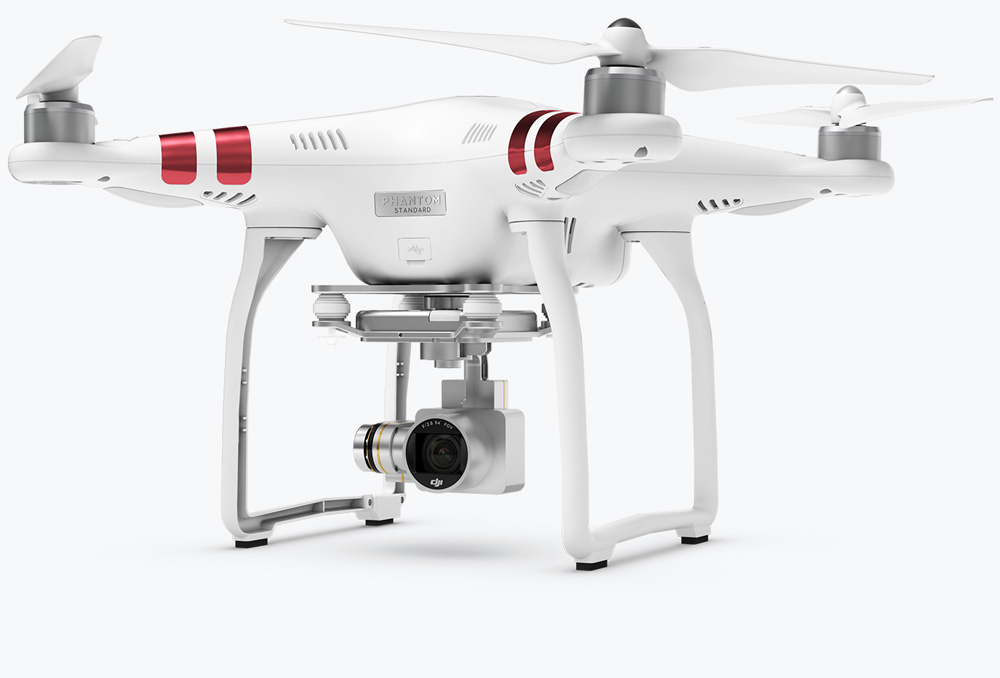
\includegraphics[width=0.7\textwidth]{images/DJI_Phantom_3_Standard.jpg}}
		\caption{DJI Phantom 3 Standard}
	\end{center}
\end{figure}

Die Drone lässt sich auf verschiedenen Wegen steuern. Es gibt die Möglichkeit der klassischen manuellen Steuerung über die Fernbedienung oder man lässt die Drone autonom fliegen. 
\newline
Allgemein ist eine App notwendig, um die Drohne zu steuern und alle Features, welche mit der Drohne kommen, zu nutzen. Hierfür stellt die Firma DJI eine eigene App, die DJI GO App zur Verfügung. Es wird aber auch ein \acf{SDK} bereitgestellt, mit dem sich eigene Apps entwickeln lassen. Durch die durch das \acl{SDK} bereitgestellten Funktionen lassen sich die Features der DJI GO App replizieren und erweitern.
\newline
Das manuelle fliegen lässt sich einfach über die mitgelieferte Fernbedienung realisieren. Die zwei Steuerknüppel dienen hierbei zur Steuerung. Die Funktion der einzelnen Steuerknüppel lässt sich über die DJI eigene App konfigurieren. Hier kann der Nutzer seine Vorlieben einstellen. 
\newline
Um die App bequem während des Fluges bedienen zu können ist an der Fernbedienung eine Halterung montiert in die man das Endgerät, auf der die App ausgeführt wird, befestigen kann. 
\newline
Der Aufbau der Fernbedienung ist in folgender Abbildung zu sehen.
\begin{figure}[H]
	\begin{center}
		{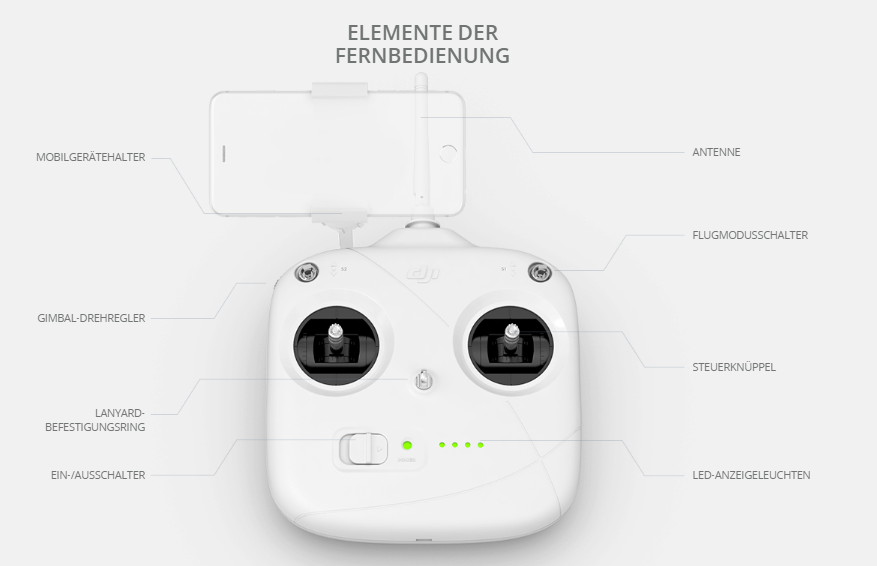
\includegraphics[width=0.5\textwidth]{images/DJI_Fernbedienung.png}}
		\caption{DJI Phantom 3 Standard - Fernbedienung}
	\end{center}
\end{figure}
Die zweite Möglichkeit ist, die Drohne autonom fliegen zu lassen. Hierbei werden sogenannte Waypoints einer Mission hinzugefügt, welche gestartet wird. Die Waypoints beinhalten die Koordinaten mit Längengrad und Breitengrad, sowie der Flughöhe und weiteren Informationen, wie der Fluggeschwindigkeit oder dem Radius mit welchem der Punkt umflogen werden soll. Um den autonomen Flug zu starten wird die Mission gestartet. Während des Fluges erkennt die Drohne über die Kamera Hindernisse und vermeidet eine Kollision mit diesen. 
\newline
Hierbei spielt das \acf{GPS} der Drohne eine wichtige Rolle. Das intelligente System merkt sich den Startpunkt der Drohne. Je nach Einstellung kehrt die Drohne automatisch zum Startpunkt zurück, sollte der Akkustand eine bestimmte Grenze unterschreiten, die Drohne außer Reichweite der Fernbedienung sein oder die return-to-home-Funktion ausgeführt wird.

Die folgende Tabelle gibt eine Übersicht über die wichtigsten, für diese Arbeit relevanten technischen Daten.
\newline
\begin{table}[H]
	\begin{center}
		\begin{tabular}{cc}
			Gewicht & 1216g \\ 
			Diagonale Größe & 350mm \\ 
			max. Steiggeschwindigkeit & 5$\frac{m}{s}$ \\ 
			max. Sinkgeschwindigkeit & 3$\frac{m}{s}$ \\ 
			max. Fluggeschwindigkeit & 16$\frac{m}{s}$ \\
			max. Flughöhe über NN & 6000m \\
			max. Flugzeit & ca. 25 min \\
			Betriebstemperatur & 0° bis 40°C \\
			Positionsbestimmung & GPS \\
			max. Sendereichweite & \begin{tabular}{c}
				FCC: 1000m \\
				CE: 500m \\
				Flughöhe: 120m
			\end{tabular}
		\end{tabular}
	\end{center}
	\caption{DJI Phantom 3 Standard - technische Daten}
\end{table}

\subsection{iPad 3}
Um die in dieser Arbeit zu erstellende App auszuführen und das Produkt zu testen ist ein mobiles Endgerät notwendig. 
\newline
Bei dem mobilen Endgerät handelt es sich um ein iPad der 3. Generation von der Firma Apple.
\newline 
Das iPad hat die Abmessungen:
\begin{itemize}
	\item Höhe: 241,2 mm
	\item Breite: 185,7 mm
	\item Tiefe: 9,4 mm
	\item Gewicht: 652 g
\end{itemize}
Die Bedienfläche ist ein 9,7" großer Multi-Touch Display. Das iPad ist \acl{WLAN} fähig und kann eine Bluetooth Verbindung aufbauen.
\begin{figure}[H]
	\begin{center}
		{\includegraphics[width=0.5\textwidth]{images/iPad3.jpg}}
		\caption{iPad 3}
	\end{center}
\end{figure}


\section{iOS-Appentwicklung}\label{sec:ioS-Appentwicklung}
Bei der Appentwicklung für iOS Geräte bietet sich die Apple eigene Programmiersprache Swift an, welche für die in dieser Arbeit erstellten App auch verwendet wurde. 
\newline
Die Entscheidung für ein für das Projekt sinnvolles Design-Pattern fiel auf das \acf{MVC} Pattern.
\newline
Für die Ansteuerung der DJI-Drone ist das DJI-SDK notwendig, sowie für die Einbindung externer Bibliotheken ist Wissen über Cocoa Pods notwendig.
\newline
Im folgendem werden die genannten Grundlagen in einzelnen Unterkapiteln kurz beschrieben.

\subsection{\acf{MVC}}\label{subsec:MVC}
Das \acs{MVC}-Pattern besteht, wie der Name sagt, aus drei verschiedenen Teilen. Dem Model, dem Controller und der View.
Das Model dient ausschließlich zur Speicherung von Daten. Zum Beispiel werden aktuelle Daten der Anwendung, wie zum Beispiel eine Flugroute in einem Model abgespeichert.
Die View ist für die Darstellung der Inhalte und Daten zuständig. Ebenso ist die View dafür zuständig die Eingaben eines Nutzers an den entsprechenden Controller weiterzuleiten. Die View beinhaltet auch die gesamte \acf{GUI}. 
Der Controller beinhaltet die Anwendungslogik und ist für die Steuerung der Anwendung verantwortlich.
\newline
\begin{figure}[H]
	\begin{center}
		{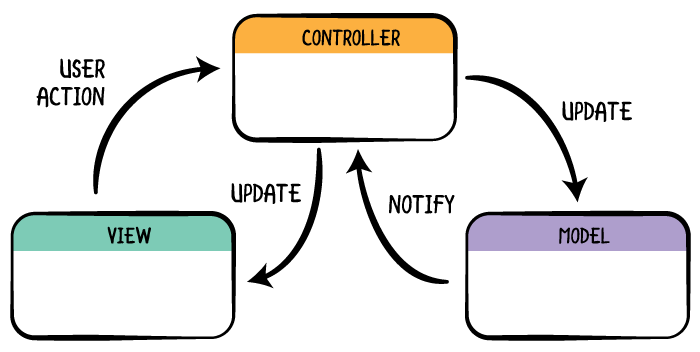
\includegraphics[width=0.5\textwidth]{images/diagram-mvc.png}}
		\caption{MVC Design-Pattern Diagramm \cite{mvc1}}
	\end{center}
\end{figure}
Das \acs{MVC} Pattern kann verschieden streng implementiert werden. In dieser Arbeit wird das Pattern in einer leichten Form angewendet. Es wird sich nicht exakt an die Spezifikation aus der Literatur gehalten.
\newline
\newline
Eine mit Xcode und Swift gschriebenen App hat als Kern eine UIApplication-Klasse. Diese Klasse verarbeitet die Interaktion zwischen System und Objekten der App. Sie verwaltet die geöffneten Views und leitet Ereignisse durch Nutzereingaben oder vom System kommend an die entsprechenden Controller weiter. 
\newline
Die \textit{ViewController} Objekte stellen in einer iOS-Anwendung die Controller des \acs{MVC} Patterns dar. Eine \textit{ViewController}-Klasse verarbeitet Nutzereingaben und aktualisiert die View. 
\newline
Die View ist in der iOS-Programmierung durch sogenannte Storyboards realisiert. 

\subsection{Cocoa}
\subsubsection{\acf{API}}
Cocoa ist eine \acf{API} zur Programmierung unter den \acf{OS} MacOS. Für die Apple \acs{OS} von mobilen Endgeräten, welche über Touch-Displays verfügen, wurde die Cocoa \acs{API} zur CocoaTouch \acs{API} erweitert. CocoaTouch beinhaltet Funktionen für die Nutzereingabe über Eingaben durch Gesten. Somit wird für die Entwicklung von iOS Apps, wie in dieser Arbeit, die CocoaTouch \acs{API} verwendet.
\newline
Die Entwicklung für Apps mit der Cocoa \acs{API} erfolgt mit den Apple eigenen Developer Tools, Xcode, welches im nächsten Kapitel beschrieben wird, und dem Interface Builder. 
\newline
Die hauptsächlich für die \acs{API} gedachten Programmiersprachen sind Objective-C und die Apple eigene Programmiersprache Swift. Die Programmierung in C und C++ ist generell auch möglich. 
\newline
Der Aufbau von Cocoa ist im Allgemeinen einfach gehalten. Cocoa besteht aus drei verschiedenen Frameworks.
\begin{itemize}
	\item \textit{Foundation}: beinhaltet alle relevanten Basisklassen, wie Strings, Arrays, Iterators, et cetera.
	\item \textit{AppKit}: stellt Klassen zur Entwicklung von \acf{GUI} zur Verfügung. Zum Beispiel Buttons, Labels, Menüs, usw..  
	\item \textit{Core Data}: dient zur Erstellung von Objektgraphen.
\end{itemize}
Klassen des Cocoa-Frameworks sind im Quellcode durch die Buchstaben \emph{NS} im Objektnamen zu erkennen. 
\subsubsection{Pods}
CocoaPods ist ein application level dependency manager für Objective-C, Swift und andere Programmiersprachen, welche in XCode laufen. Pods stellt ein Standardformat zum managen von externen Bibliotheken bereit.
\newline
Die Projektabhängigkeiten werden mittels Podfile-Dateien in einem Projekt beschrieben. Im Folgendem ist ein Beispiel zu sehen.
\newline
\begin{lstlisting}[language=ruby, caption={Podfile Beispiel}]
	# platform: iOS, '9.0'
	use_frameworks!
	project 'AirQualityDrone.xcodeproj'
	target 'AirQualityDrone' do
	pod 'DJI-SDK-iOS' '~> 4.4'
	pod 'DJI-UILibrary-iOS', '~> 4.4'
	pod 'CocoaAsyncSocket'
	pod 'DTMHeatmap'
	end
\end{lstlisting}
Um die externen Bibliotheken zu installieren, wird der Befehl \textit{pod install} aufgerufen. Dadurch werden die Quellen der Bibliotheken geladen und das Projekt in Xcode eingerichtet, sodass die Bibliotheken separat gebaut werden. In das Projekt werden die Dateien über eine statische Bibliothek (\textit{libPods.a}).
\begin{figure}[H]
	\begin{center}
		{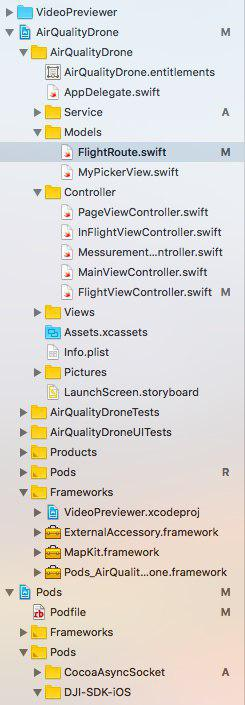
\includegraphics[width=0.5\textwidth]{images/pods.jpg}}
		\caption{Externe Bibliotheken in Xcode}
	\end{center}
\end{figure}

\subsection{Xcode}
Xcode ist eine \acl{IDE} von Apple für das \acs{OS} macOS. Xcode ist für die Entwicklung von Programmen und Apps für macOS, iOS, tvOS und watchOS gedacht. 
Die \acs{IDE} ist BEstandteil der Xcode Tools. 
\newline
Die Xcode Tools beinhalten:
\begin{itemize}
	\item Xcode \acs{IDE}
	\item Interface Builder
	\item Instruments
	\item Xcode Core
	\item Dashcode
	\item Quanz Composer
	\item iPhone Simulator
\end{itemize}
Die iOS App, welche Bestandteil dieser Arbeit ist, wird ausschließlich mit Xcode entwickelt.
Die folgende Abbildung zeigt eine Übersicht der Xcode-Oberfläche.
\begin{figure}[H]
	\begin{center}
		{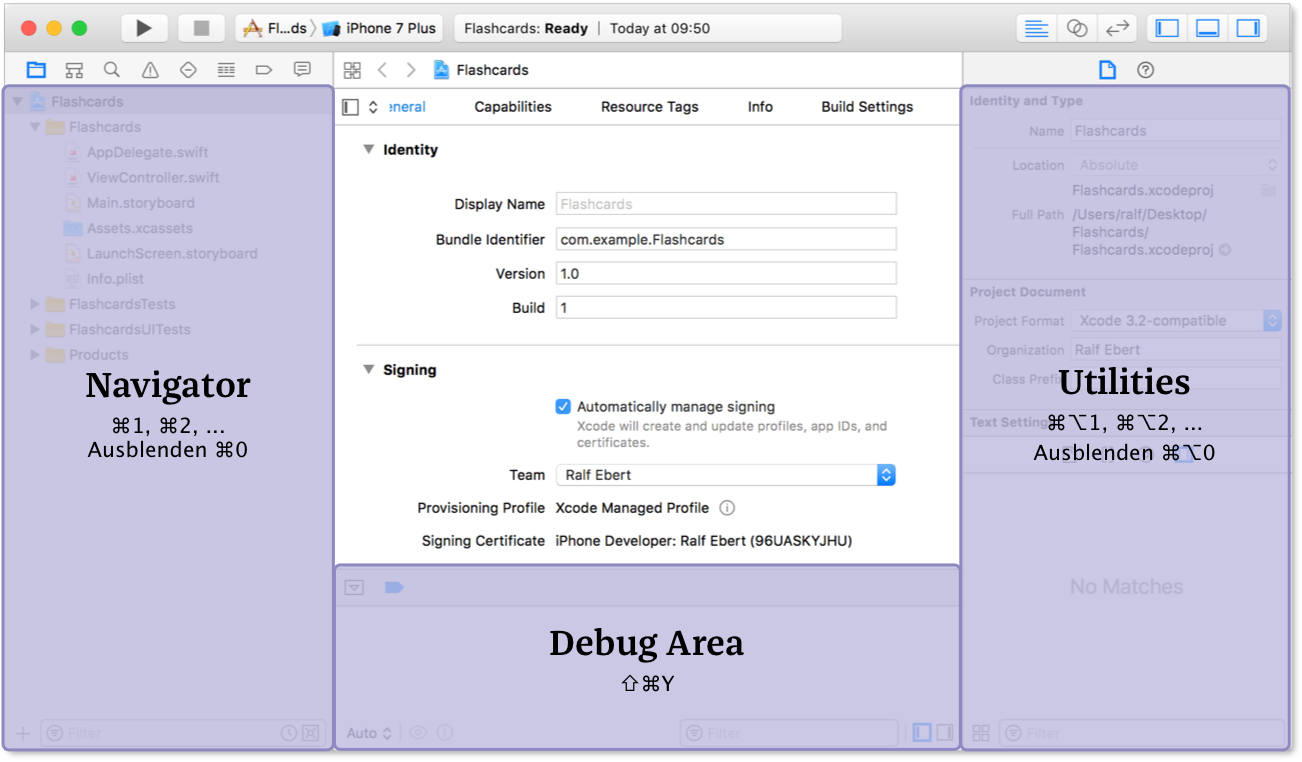
\includegraphics[width=0.8\textwidth]{images/xcode_views.png}}
		\caption{Xcode-Oberfläche}
	\end{center}
\end{figure}
Zentral ist in Xcode der Editor zu finden. Auf der linken Seite befindet sich der Navigator. Unterhalb des Editors befindet sich die Debug Area und auf der rechten Seite die Utilities. Navigator, Debug Area und Utilities lassen sich über die Buttons in der oberen rechten Ecke ausblenden und ermöglichen es so das Editor Fenster größer zu machen.
\newline
Die Projektstruktur ist in Abbildung 2.5 zu sehen. 

\subsection{SWIFT}\label{subsec:SWIFT}
Swift ist eine Programmiersprache des Technik Konzerns Apple. Sie wurde für die Entwicklung von Apps für iOS, Mac, Apple TV und Apple Watch kreiert. Swift ist kostenlos und Open Source. Die Sprache steht unter der Apache 2.0 Open Source Lizenz. Somit kann eine große Community direkt zum Swift Quellcode beitragen. 
\newline
Swift vereint unterschiedliche Konzepte verschiedener Programmiersprachen, wie zum Beispiel Objective-C und Python. Dies führt dazu, dass Sie sich durch Paradigmen wie objektorientiert und imperativ beschreiben lässt. Swift greift Mechanismen, wie Klassen, Vererbung, Closures, Typinferenz, generische Typen, etc., auf, welche von anderen Programmiersprachen bereits bekannt sind. 
\newline
Für die Appentwicklung wurde die Programmiersprache Swift unter der Version 4.1 verwendet. 

\subsection{DJI-\acf{SDK}}\label{subsec:DJI-SDK}
DJI bietet neben dem Verkauf von Drohnen auch noch andere Leistungen an. Hierzu gehören diverse \acs{SDK}, die die Entwicklung von Apps und Programmen für die Drohnen von DJI erleichtern. 
\acs{SDK} die angeboten werden sind:
\begin{itemize}
	\item Mobile SDK
	\item Onboard SDK
	\item Guidance SDK
	\item Payload SDK
\end{itemize}
In dieser Arbeit ist nur das Mobile SDK relevant. 
\newline
Das DJI Mobile SDK unterstützt die Plattformen iOS 9.0 oder höher, sowie Android 5.0.0 oder höher. Da das mobile Endgerät mit einem iOS \acs{OS} läuft, wird in dieser Arbeit die Ausführung des DJI Mobile SDK für iOS verwendet. Hierbei ist die Programmierung in den Sprachen Swift und Objective-C möglich. Wie im Kapitel 2.3.4 erwähnt wird in dieser Arbeit die Programmiersprache Swift 4.1 verwendet. 
\newline
Das SDK bietet verschiedene Kernfunktionalitäten an. Zu diesen wichtigen und nützlichen Features gehört die Obstacle avoidance,  High and low level flight control, Aircraft state through telemetry and sensor data, Live video feed, Pre defined missions, wie Waypoint, HotPoint oder FollowMe und State information und control of Battery und Remote Controller. 
\newline
Für die Entwicklung von \acs{GUI} stellt DJI eine UXLibrary zur Verfügung, welche graphische Elemente für die wichtigsten Funktionen des mobile \acs{SDK} bereitstellt.

